\documentclass{article}

%change 
% Language setting
% Replace `english' with e.g. `spanish' to change the document language
\usepackage[english]{babel}

% Set page size and margins
% Replace `letterpaper' with`a4paper' for UK/EU standard size
\usepackage[letterpaper,top=2cm,bottom=2cm,left=3cm,right=3cm,marginparwidth=1.75cm]{geometry}

% Useful packages
\usepackage{amsmath}
\usepackage{graphicx}
\usepackage[colorlinks=true, allcolors=blue]{hyperref}

\title{Cash-flow maturity and risk premia in CDS markets.}
\author{Antonio Pineda Acosta, Nidhi Beeravolu, Kausthub Keshava and Diana Castellanos Polina}

\begin{document}
\maketitle

\begin{Data science tools for finance final project}
Professor: Jeremy Bejerano.
\end{abstract}

\section{Introduction}

The present project is an academic exercise designed to replicate and analyze the Credit Default Swap (CDS) returns specified by \cite{kelly2017}. The dataset, sourced from the comprehensive repositories of Markit, provides the empirical foundation upon which our replication model is constructed. This model is designed to not only corroborate the work of \cite{kelly2017} but also to substantiate the theoretical implications proposed by \cite{Palhares2013} concerning the maturation of cash-flows and their correlation with the risk premia observed in the market for credit default swaps.
This project is committed to the application of rigorous methodological practices to ensure the fidelity of the replication process. It is the intention of this study to contribute to the existing body of knowledge on CDS market mechanisms, offering nuanced insights into the determinants of risk premia as influenced by the maturity structure of cash flows.


\section{CDS Returns definition and variables}

In particular, let $CDS_t$ be the credit spread at day $t$. The one-day return on a short CDS strategy (in the case of no default) is
\begin{equation}
CDS^{ret}_t = \frac{CDS_{t-1}}{250} + \Delta CDS_t \times RD_{t-1}.
\end{equation}
The first term on the right-hand-side is the carry component of the return due to the seller's receipt of insurance premium payments. The second term is the capital gain return, equal to the change in spread times the lagged risky duration of the contract (denoted $RD_{t-1}$) \cite{sourcekey}.


According to \cite{kelly2017}, 
%talk about the definition and what we are going to do

\section{CDS returns estimation}
In this section we will present the data we are going to use and the estimation of the CDS returns.

\subsection{Data}

%PROFESSOR INSTRUCTION: explain the data sources that you used. The LaTeX document should not contain code snippets, 
%but only give the tables and charts and a high level discussion of the project.

% Rates, 
% Risky dutarion
% CDS spreads


First you have to upload the image file from your computer using the upload link in the file-tree menu. Then use the includegraphics command to include it in your document. Use the figure environment and the caption command to add a number and a caption to your figure. See the code for Figure \ref{fig:myplot} in this section for an example.

Note that your figure will automatically be placed in the most appropriate place for it, given the surrounding text and taking into account other figures or tables that may be close by. You can find out more about adding images to your documents in this help article on \href{https://www.overleaf.com/learn/how-to/Including_images_on_Overleaf}{including images on Overleaf}.

\begin{figure}
\centering
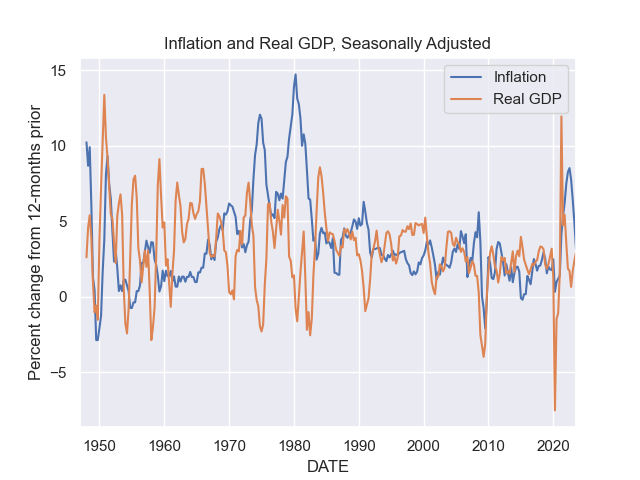
\includegraphics[width=0.75\textwidth]{../output/example_plot.png}
\caption{\label{fig:myplot}This image was uploaded via the file-tree menu.}
\end{figure}

\subsection{Estimation}

%PROFESSOR INSTRUCTION: You should give a high level overview of how the replication project went. 
%Where did you find success, where were the challenges? 


\section{Conclusion}

Comments can be added to your project by highlighting some text and clicking ``Add comment'' in the top right of the editor pane. To view existing comments, click on the Review menu in the toolbar above. To reply to a comment, click on the Reply button in the lower right corner of the comment. You can close the Review pane by clicking its name on the toolbar when you're done reviewing for the time being.

Track changes are available on all our \href{https://www.overleaf.com/user/subscription/plans}{premium plans}, and can be toggled on or off using the option at the top of the Review pane. Track changes allow you to keep track of every change made to the document, along with the person making the change. 

\subsection{How to add Lists}

You can make lists with automatic numbering \dots

\begin{enumerate}
\item Like this,
\item and like this.
\end{enumerate}
\dots or bullet points \dots
\begin{itemize}
\item Like this,
\item and like this.
\end{itemize}

\bibliographystyle{alpha}
\bibliography{bibliography}

\end{document}